\subsection{Overview}
The system to be designed needs to help customers make reservations in their favourite shops in the least amount of time possible and also keep track of all the future appointments they have taken.\\
It also must allow shop owners to register their establishment to the platform and keep track of the next customers that have registered an appointment.\\
Since this interaction between user and system can be summarize as:
\begin{enumerate}
	\item User request a service to the system.
	\item System responds to the user with the requested service.
\end{enumerate}
Based on this, a client-server architectural approach has been chosen.
\begin{figure}[H]
	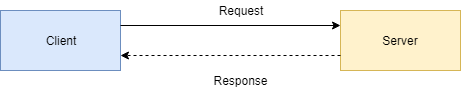
\includegraphics{Img/ClientServerArchitecture}
	\caption{Client Server architecture}
	\label{fig:clientserver}
\end{figure}
\noindent Furthermore, the system can be divided into three different subsystems: the presentation layer, the application layer and the data layer, where: 
\begin{itemize}
	\item The \emph{Presentation Layer} provides the GUI of the system.
	\item The \emph{Logic Layer} contains the logic of the application,that receives the requests from the user.
	\item The \emph{Data Layer} stores and maintains the data needed from the system to works properly, i.e. user's \& shop's information and reservations details.
\end{itemize}
\subsection{Model–View–ViewModel (MVVM)}
Since in the Android development it's quite easy to find conflicting arguments regarding the use of the well known Model-View-Controller pattern due to views being in part also controllers, the officially suggested architecture is the Model–View–ViewModel one, where the (graphical user interface) GUI is separated from the model by a ViewModel that handles the conversion of data and exposes to the View only the needed information.\\
The main advantage of using ViewModel classes is that they are part of the Android class system already, therefore the developer only needs to extend the ViewModel class to create a custom one for the needed purpose.\\
It should be noted how ViewModel classes are not destroyed when the View is recreated (for example when rotating the screen), meaning that data is actually preserved to allow for a better user experience.\\
A classic example of MVVM can be seen when using \textbf{Room} to locally store data in a MySQL database (with all the advantages of the latest Repository and DAO integration for easier use), but for this project there was no need to do so since Firebase already takes care of storing data when off-line.
\clearpage
\subsection{Live Data}\vspace{-0.1cm}
Live Data is a class of objects that allow to be observed, meaning that if a ViewModel returns a reference to a Live Data Object, the View can simply observe the given object and when a change happens it can update itself by executing the code in the call.This has been used in conjunction with FirebaseFirestore observers to update the reservation lists in real time even when the application is already opened, making therefore obsolete the use of a "refresh button".
\subsection{Component View}
\subsubsection{Overview}
In \autoref{fig:hlCD} is possible to see the high level components of the system and the interfaces used to connect one to another, where:
\begin{itemize}
\item \emph{Firebase} allows the use of many functionalities to aid development;
\item \emph{Data} is a macro category containing functionalities and services to store information:
\begin{itemize}
\item \emph{Firestore} is the cloud database system used to store information.
\item \emph{Real-time DB} is the database used to store chat conversations.
\item \emph{Storage} is Firebase system to store files such as user's profile pictures.
\end{itemize}
\item \emph{Firebase Auth} provides the authentication system;
\item \emph{Cloud Functions} allow to make modifications to the database when defined triggers are fired, moving computation to the back-end instead of relying on the user's device;
\item \emph{Cloud Messaging} notification system handled by the back-end once properly set-up;
\item \emph{Maps API} given by Google to use Maps functionalities such as address search and maps display;
\item The \emph{Mobile Application} is the mobile application used by a user with his/her smartphone.
\end{itemize}
\begin{figure}[H]
\centering
	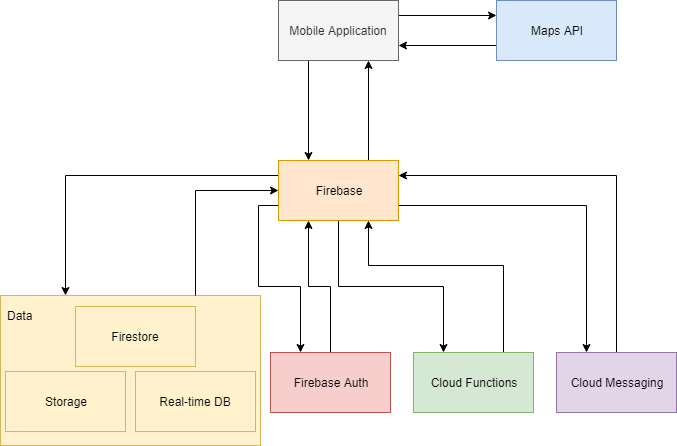
\includegraphics[width = 0.75\textwidth, keepaspectratio = true]{Img/HighLevelComponent}
	\caption{High level Component Diagram}
	\label{fig:hlCD}
\end{figure}
\clearpage
\subsubsection{Firestore View}
Unlike traditional Entity-Relationship DB systems, Firestore is organized in Collections-Documents hierarchy that can be further nested, meaning a Document can contain one or more Collections containing other Documents and so on.\\
The main Collections used are shown in \autoref{fig:HighLevelDB}, while the others shown in \autoref{fig:HighLevelDBSupport} where used as support Collections in order to add functionalities.

\begin{figure}[H]
\centering
	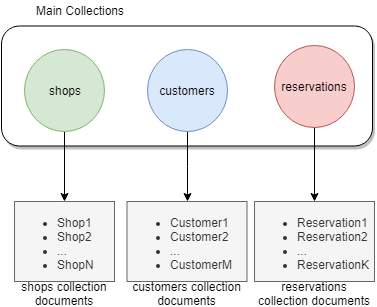
\includegraphics[width = 0.8\textwidth, keepaspectratio = true]{Img/HighLevelDB}
	\caption{\emph{Main} Collections}
	\label{fig:HighLevelDB}
\end{figure}

\begin{figure}[H]
\centering
	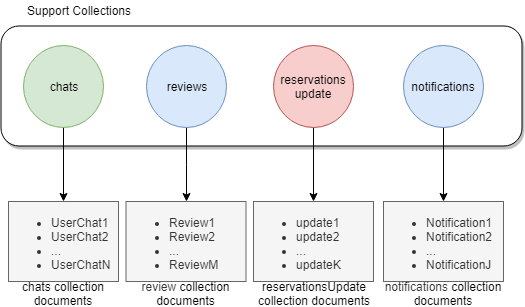
\includegraphics[width = 0.8\textwidth, keepaspectratio = true]{Img/HighLevelDBSupport}
	\caption{\emph{Support} Collections}
	\label{fig:HighLevelDBSupport}
\end{figure}
\clearpage
\noindent Each object is stored in its separate document with an unique ID (UID) given by Firestore itself, here are some examples of how each one looks like in the JSON representation:

\lstset{
    string=[s]{"}{"},
    stringstyle=\color{blue},
    comment=[l]{:},
    commentstyle=\color{black},
escapeinside={\\*}{*\\},    
}
\paragraph*{Customer}:
\label{Par:Customer}
\begin{lstlisting}
{
  "uid": "jcUgNG7wi4eZmQjakQRTQNSYWqk1",
  "name": "Bob Peterson",
  "phone": "3343200266",
  "mail": "bob.peterson@gmail.com",
  "profilePicUrl": "URL to storage" \*\textcolor{ForestGreen}{File storage is a different service}*\\
}
\end{lstlisting}
\paragraph*{Shop}:
\label{Par:Shop}
\begin{lstlisting}
{
  "uid": "0wiQ9FYr1YdL1aTPVgUe5ndCmSt2",
  "name": "Forbici & Capelli",
  "phone": "0523468159",
  "mail": "forbici.capelli@gmail.com",
  "profilePicUrl": "URL to storage", \*\textcolor{ForestGreen}{File storage is a different service}*\\
  "address": "Via Emilia Parmense 22/B",
  "city": "Piacenza",
  "zip": "29122",
  "latitude": 45.0391566,
  "longitude": 9.7204521,
  "intLongitude": 9,
  "averageReviews": 4.7,
  "numReviews": 12,
  "tags": ["barber", "parrucchiere", "forbici & capelli", "forbici", "capelli"],
  "hours": [
    {
      "Monday": [
        "08:30",
        "12:00",
        "Closed",
        "Closed"
      ],
      "Tuesday": [
        "07:30",
        "12:00",
        "14:00",
        "17:30"
      ],
      "Wednesday": [
        "07:30",
        "12:00",
        "14:00",
        "17:30"
      ]\*\textcolor{ForestGreen}{Cut for page length purposes}*\\
}
\end{lstlisting}
\clearpage
\paragraph*{Reservation}:
\label{Par:Reservation}
\begin{lstlisting}
{
  "time": "1563199200000", \*\textcolor{ForestGreen}{Stored as long (time in milliseconds)}*\\
  "where": "Via Emilia Parmense 22/B",
  "shopUid": "0wiQ9FYr1YdL1aTPVgUe5ndCmSt2",
  "shopName": "Forbici & Capelli",
  "shopPic": "URL to storage", \*\textcolor{ForestGreen}{File storage is a different service}*\\
  "customerUid": "jcUgNG7wi4eZmQjakQRTQNSYWqk1",
  "customerName": "Bob Peterson",
  "customerPic": "URL to storage" \*\textcolor{ForestGreen}{File storage is a different service}*\\
}
\end{lstlisting}
\paragraph*{Chat}: \textcolor{ForestGreen}{Bob Peterson's}
\label{Par:Chat}
\begin{lstlisting}
{
  "thisName": "Bob Peterson",
  "thisPhoto": "URL to storage", \*\textcolor{ForestGreen}{File storage is a different service}*\\
  "otherName": "Forbici & Capelli",
  "otherUid": "0wiQ9FYr1YdL1aTPVgUe5ndCmSt2",
  "otherPhoto": "URL to storage", \*\textcolor{ForestGreen}{File storage is a different service}*\\
  "lastText": "See you on Monday!",
  "isRead": true,
  "lastMsgDate": "2019-08-10 13:11:17 UTC+2"
}
\end{lstlisting}
\paragraph*{Reservation Update}: \textcolor{ForestGreen}{Needed only for listeners}
\label{Par:ReservationUpdate}
\begin{lstlisting}
{
  "reservations": 2
}
\end{lstlisting}
\paragraph*{Review}:
\label{Par:Review}
\begin{lstlisting}
{
  "reviewScore": 3,
  "ShopUid": "DzSJgsPGfsPrDhAFwEnyK6VeRJH2",
  "customerUid": "jcUgNG7wi4eZmQjakQRTQNSYWqk1"
}
\end{lstlisting}
\paragraph*{Notification}: \*\textcolor{ForestGreen}{Once the notification is sent the entry will be automatically removed}*\\
\label{Par:Notification}
\begin{lstlisting}
{
  "recipientUid": "0wiQ9FYr1YdL1aTPVgUe5ndCmSt2",
  "title": "Bob Peterson", 
  "body": "See you on Monday!" \*\textcolor{ForestGreen}{Empty if it's a new reservation notification}*\\
}
\end{lstlisting}
\clearpage
\subsubsection{Real-time Database View}
\label{RealTimeDB}
For convenience the actual chat conversations are stored in the real-time database under the node \textbf{messages} in a series of sub-nodes where each conversation is identified by \textit{smallerUID\_biggerUID} (to be uniquely identifiable from both users without storing a new conversation UID) where the difference is given by the \textit{compare} method that Java offers for Strings.
Each message in a conversation is a new child node under the \textit{smallerUID\_biggerUID} generated UID with the following structure:
\dirtree{%
.1 reservation-PRIVATE\_PROJECT\_UID.
.2 messages.
.3 15dQDKOmhKTImo4nZS9Yielor2m2\_jcUgNG7wi4eZmQjakQRTQNSYWqk1.
.4 -LjhD3f7Nzuy12g\_q2LZ \textcolor{ForestGreen}{UID auto-generated}.
.5 message: "Hi, would you mind if I asked you a question?".
.5 user: "Bob Peterson".
.3 DzSJgsPGfsPrDhAFwEnyK6VeRJH2\_jcUgNG7wi4eZmQjakQRTQNSYWqk1.
.4 -MLDD3f7dxipo89s\_23aq \textcolor{ForestGreen}{UID auto-generated}.
.5 message: "Hi, how much is it for a haircut?".
.5 user: "Bob Peterson".
.4 -TjhDf5qNzuy12g\_qongZ \textcolor{ForestGreen}{UID auto-generated}.
.5 message: "It's 15 euros".
.5 user: "Forbici \& Capelli".
}
\subsubsection{Storage View}
The Firebase Storage structure is simply organized in a single folder since it's only needed to store profile pictures.
\dirtree{%
.1 profile\_pics.
.2 profile\_picture\_user\_1.
.2 profile\_picture\_user\_2.
.2 profile\_picture\_user\_3.
.2 profile\_picture\_user\_4.
}
\subsubsection{Firebase Auth View}
The Firebase Authentication system handles automatically the authentication of the connected user by storing:
\begin{itemize}
\item Identifier (for example email address)
\item Provider (Email/Gmail account/Phone etc...)
\item Creation date
\item Last sign in
\item User UID (which is then used in the DB as an identifier)
\end{itemize} 
\clearpage
\subsubsection{Firebase Cloud Functions View}
Cloud functions are functions written in JavaScript that allow for actions to be executed by the Firebase server on specific triggers to relieve computation from the user's device.\\
For this project two functions have been written:
\begin{itemize}
\item \textbf{newShopReview}: triggered when a new \textit{document.write} (which means it will trigger both on update and on create) occurs in the \textit{reviews} collection, it is tasked to read the value of the review and update the average and total number of reviews of the shop that was reviewed. It also handles the case in which the review is just an update of an already existing one.
\item \textbf{sendNotification}: triggered when a new \textit{document.create} occurs in the \textit{notification} collection, it is tasked with sending the content of the notification to the given recipient. It also handles the deletion of the created element in the database to avoid storing now useless data.
\end{itemize}
\subsubsection{Firebase Cloud Messaging View}
Built in system for messaging (notifications), since at login each user subscribes to an unique topic (identified by the UID of user itself), the Cloud Messaging system will send the notification content (by using the \textit{sendNotification} cloud function) to only that user. The notification will be received as soon as the user's device is reachable.
\subsubsection{Maps API}
Google Maps API have been added to the project in order to use the \textbf{places} and the \textbf{maps SKD for Android} that are needed respectively to search an address from where the search will start and to show the map view when a shop is selected.
\subsubsection{Mobile Application}
The \emph{Mobile Application} is used by the user via its own smart device. The \emph{Mobile Application} communicates directly with the Firebase and Google Maps system using the provided API.

\clearpage
\subsection{Implementation choices}
\label{Implementation choices}
The technology chosen for the implementation on the system are all based on Java and JavaScript since it is the most common way of developing Android applications using Firebase and the availability of documentation and other sources of learning materials are abundant, plus some experience was already obtained during past projects. \\It also offers the possibility of adding new functionalities in future, making the system more scalable given how the platform is constantly evolving\\\\
To summarize the technologies used are:
\paragraph{Mobile application:} entirely Android (Java) based with Firebase and Google Maps API added in order to use the external tools. Other modules such as RecycleViews and Cards have been added.
\paragraph{Main DBMS:} Firestore was selected over the old real time database system since it has been developed as a successor to substitute it. I provides easy to use DB mechanisms, at the loss of complexity such as complex queries and it's not a relational DB system which is usually more familiar.
\paragraph{Chat DBMS:} It has been used the real-time database because it's ideal to store simple structures like the one needed for chats and shown in \autoref{RealTimeDB}.
\paragraph{Storage:} Firebase Storage system has been chosen since it's part of the ecosystem.
\paragraph{Cloud Functions:} Just like Storage, Firebase Cloud Functions have been chosen since they are already part of the ecosystem and they were needed for some back-end actions.
\paragraph{Authentication:} Firebase auth allows for easy and fast authentication methods already handled.
\paragraph{Cloud Messaging:} Part of the Firebase ecosystem, handles the majority of the work needed to deliver notifications to users.
\clearpage
\subsection{Runtime View}
Here are represented the two most important runtime views by using diagrams that highlight the main actions the user has to follow in order to complete the given task.\\
In \autoref{fig:RegistrationDiagram} it's highlighted in red the interaction that the system has with the authentication system, then the two branches between choosing to register as a customer (green) or shop (blue) are available to be picked.\\
In \autoref{fig:ReservationDiagram} are again highlighted in red the interactions of the application with the Firebase systems, the yellow one is referred to the use of Google Maps API (in this case the \textbf{places} API to be exact) while in blue is noted the optional choice to select a different distance than the default one.\\
It should be noted how none of the handled errors or problems are shown to keep the diagrams simple.

\begin{figure}[H]
  \centering
  \begin{minipage}[b]{0.45\textwidth}
    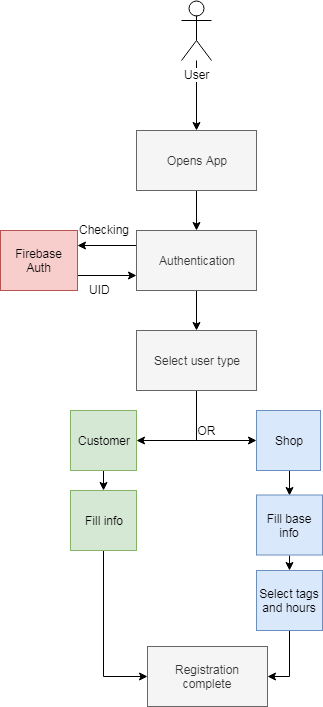
\includegraphics[width=\textwidth]{Img/RegistrationDiagram}
	\caption{\emph{User} registration diagram}
	  \label{fig:RegistrationDiagram}
  \end{minipage}
  \hfill
  \begin{minipage}[b]{0.45\textwidth}
    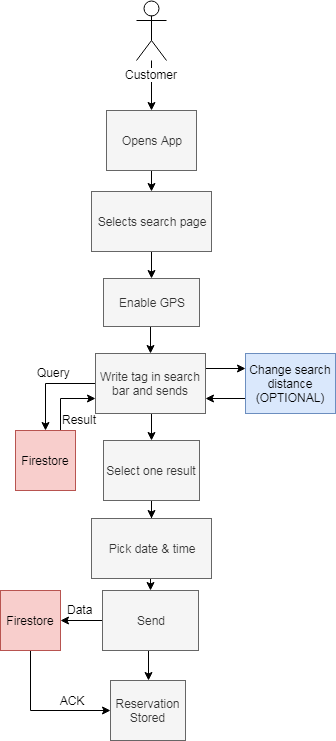
\includegraphics[width=\textwidth]{Img/ReservationDiagram}
	\caption{\emph{Customer} reservation process}
	  \label{fig:ReservationDiagram}
  \end{minipage}
\end{figure}














